\chapter{固定拓扑持续智能的统一闭环与复杂可解问题的可解原理}
\label{chap:fixed-topology-solvability}

\section{问题的提出：有限认知主体为什么仍可能解决任意复杂的可解问题}

前述各章已经逐步构造出一个具有持续主体、三相记忆、自我连续性、运行时自调节、认知负载治理、认知边界与外部卸载能力的固定功能拓扑智能体。其核心状态可以抽象为
\begin{equation}
\mathcal A_t
=
\left(
h_t,
E_t,
\Theta_t,
\Psi_t,
\Omega_t,
a_t,
G_t,
\mathcal M_t
\right),
\end{equation}
其中，$h_t$ 为当前工作记忆状态，$E_t$ 为情景轨迹结构，$\Theta_t$ 为长期生成结构，$\Psi_t$ 为自我与身份慢结构，$\Omega_t$ 为生命周期生成吸引子，$a_t$ 表示 AHC 内稳态调制状态，$G_t$ 表示当前目标结构，$\mathcal M_t$ 则表示 Agent 可以访问的内部与外部认知载体集合。

与此同时，Agent 的工作记忆存在有限容量约束。若以 $W$ 表示可稳定维持的工作记忆有效容量，则在任意时刻存在
\begin{equation}
C_{\mathrm{run}}(t)
\leq
C_{\max}(W),
\label{eq:wm-capacity}
\end{equation}
其中 $C_{\mathrm{run}}(t)$ 表示当前必须在显式认知表面 $h_t$ 中同步维持的有效关系结构负载。

这一条件立即产生一个看似根本性的悖论：

\begin{statementbox}
\centering
\adjustbox{max width=.96\linewidth}{\(\displaystyle \text{有限的 }h_t
\quad\Longrightarrow\quad
\text{是否只能解决有限复杂度的问题？}\)}
\end{statementbox}

如果答案为肯定，那么一个具有有限工作记忆的 Agent 无论拥有多少长期记忆、工具和外部环境，都无法真正面对开放世界中的复杂任务。然而，人类智能以及成熟的软件系统所展示的现象恰恰相反：局部认知容量是有限的，但系统能够通过分解、记忆、外化、程序化、工具化和时间展开处理远超过单次工作记忆容量的问题。

因此，本章所研究的不是一个无限计算能力的理想主体，而是如下问题：

\begin{statementbox}
\centering
\adjustbox{max width=.96\linewidth}{\(\displaystyle \text{在 }C_{\mathrm{run}}(t)\leq C_{\max}(W)
\text{ 始终成立的条件下，}
\text{一个持续 Agent 能解决多大的问题类？}\)}
\end{statementbox}

本章将证明一个条件性的完备性结论：

\begin{quote}
一个具有有限工作记忆，但拥有可持续的三相记忆、任务分解、认知调度、结构压缩、边界管理、外部卸载、工具调用、现实验证以及可恢复执行能力的 Agent，并不要求在任意一个时刻同时承载整个问题结构。对于满足有限可表示、可递归分解、可验证和资源可达等条件的复杂可解问题，整体复杂度可以被重新分布到时间、长期记忆、外部载体、工具和环境中，使任何单个认知时刻只承担有限的局部结构。因此，有限工作记忆并不构成复杂可解问题可解性的原则性障碍。
\end{quote}

需要首先强调，本章所证明的并不是 ``AgentOS 能够在有限时间和有限资源内解决任何数学上可计算的问题''。这在一般意义上是不可能成立的。本章建立的是一个相对于明确定义的问题类、资源闭包与接口条件的\emph{条件可解性定理}。该区分是整个理论保持数学严谨性的必要前提。

\begin{figure}[htbp]
\centering
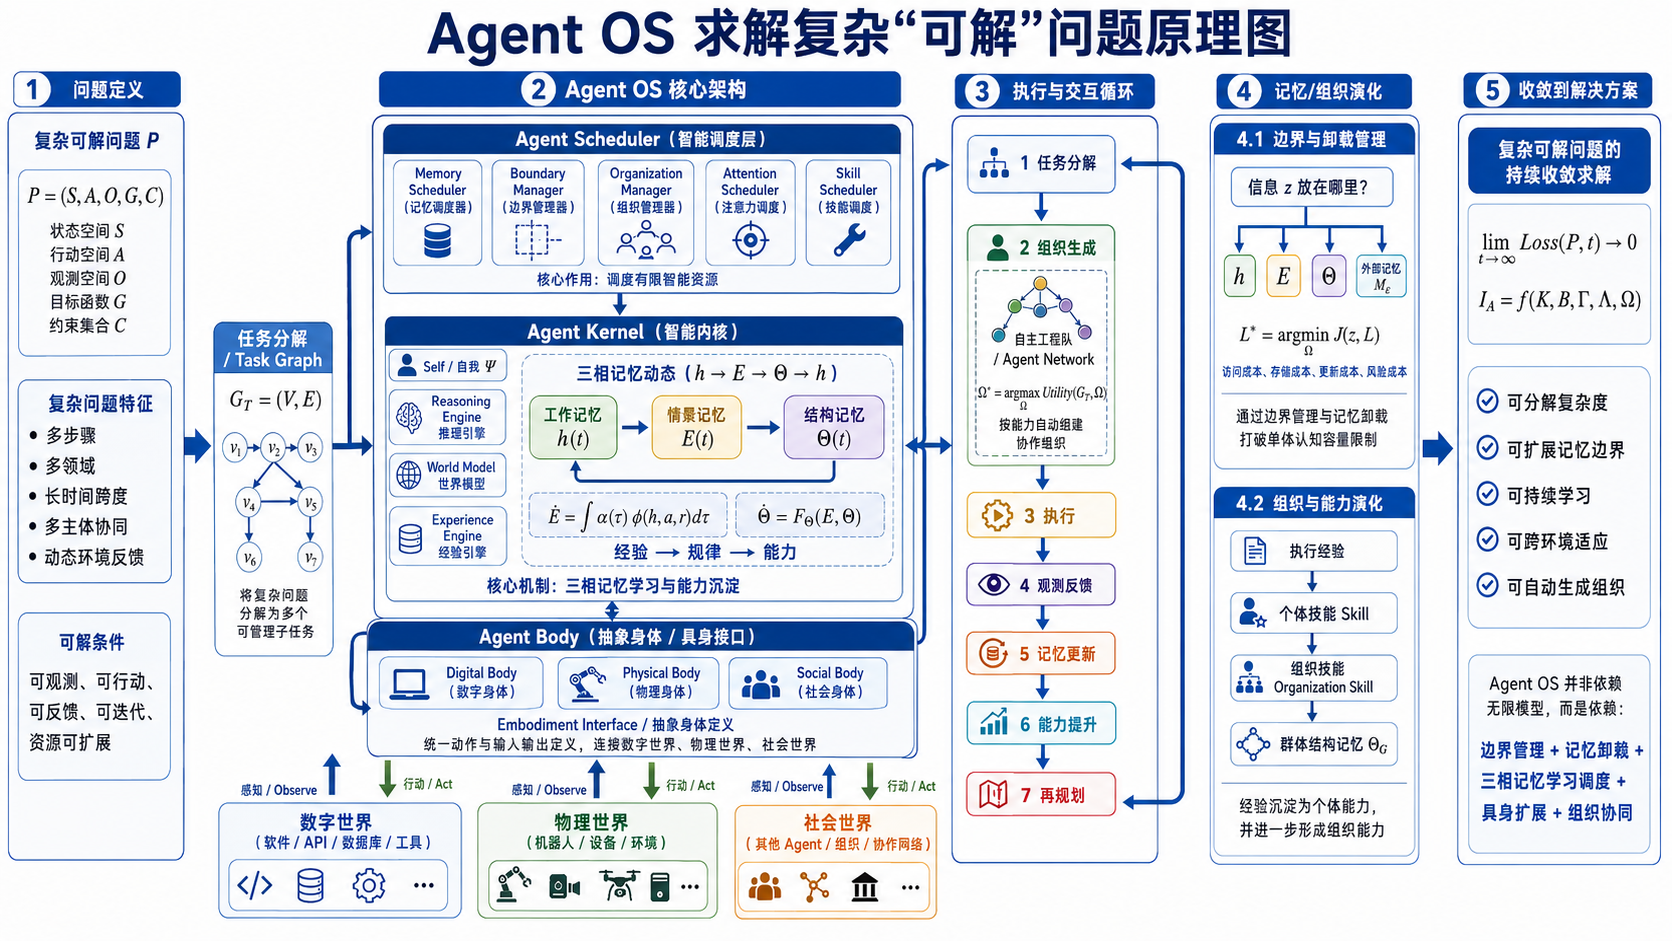
\includegraphics[width=.9\textwidth,height=.38\textheight,keepaspectratio]{images/semantic-modulation-safety-channels.png}
\caption{持续Agent求解复杂可解问题的闭环原理示意图}
\end{figure}


\section{复杂可解问题的形式定义}

为了讨论“复杂可解问题”，首先定义一个交互式问题
\begin{equation}
\Pi
=
\left(
\mathcal X,
\mathcal U,
\mathcal O,
F,
H,
x_0,
\mathcal G,
\mathcal C
\right),
\end{equation}
其中：

\begin{itemize}
    \item $\mathcal X$ 为真实世界状态空间；
    \item $\mathcal U$ 为 Agent 可执行行动空间；
    \item $\mathcal O$ 为可获得观测空间；
    \item $F$ 为世界状态转移关系；
    \item $H$ 为观测映射；
    \item $x_0$ 为初始现实状态；
    \item $\mathcal G\subseteq\mathcal X$ 为目标状态集合；
    \item $\mathcal C$ 为安全、资源、逻辑和物理约束集合。
\end{itemize}

世界按照
\begin{equation}
x_{t+1}
=
F(x_t,u_t,\xi_t)
\label{eq:world-dynamics}
\end{equation}
演化，其中 $\xi_t$ 表示环境扰动或未知变量，Agent 获得
\begin{equation}
o_t
=
H(x_t)+\nu_t,
\end{equation}
其中 $\nu_t$ 表示观测噪声。

一个策略 $\pi$ 根据 Agent 当前可获得的信息历史产生行动：
\begin{equation}
u_t
=
\pi(\mathcal I_t).
\end{equation}

如果存在一个有限描述的策略 $\pi^\star$，使得在给定约束 $\mathcal C$ 下，系统能够以规定的成功意义到达 $\mathcal G$，则称问题 $\Pi$ 为\emph{可解问题}。确定性情况下可写为
\begin{equation}
\exists \pi^\star,\exists T<\infty:
\quad
x_T\in\mathcal G,
\end{equation}
并且
\begin{equation}
(x_t,u_t)\models\mathcal C,
\qquad
0\leq t\leq T.
\end{equation}

对于随机或部分可观测环境，则可以相应要求
\begin{equation}
\Pr_\pi(x_T\in\mathcal G)
\geq
1-\delta,
\end{equation}
或者采用期望损失条件
\begin{equation}
J(\pi)
=
\mathbb E
\left[
\sum_{t=0}^{T}
\ell(x_t,u_t)
\right]
\leq
J_{\max}.
\end{equation}

问题的\emph{复杂性}并不由一个单一标量完全刻画。更一般地，可将其表示成
\begin{equation}
\mathfrak C(\Pi)
=
\left(
C_{\mathrm{rel}},
C_{\mathrm{temp}},
C_{\mathrm{branch}},
C_{\mathrm{unc}},
C_{\mathrm{ctrl}},
C_{\mathrm{resource}}
\right),
\end{equation}
分别表示关系结构复杂度、时间依赖复杂度、搜索分支复杂度、不确定性、控制耦合程度以及资源需求。

因此，一个问题完全可能满足
\begin{equation}
C_{\mathrm{total}}(\Pi)
\gg
C_{\max}(W),
\end{equation}
同时仍然具有一个可被有限步骤实现的解。

问题的总复杂度大于工作记忆容量，并不等价于问题在任意时刻都要求同时维持同样大的活跃结构。

这一区别是整个可解原理的出发点。

\section{瞬时复杂度与生命周期复杂度的分离}

定义问题生命周期中的完整结构集合为
\begin{equation}
\mathcal C_\Pi
=
\left\{
C_1,
C_2,
\ldots,
C_N
\right\},
\end{equation}
其中 $C_i$ 为问题相关 CSO。

Agent 在时刻 $t$ 实际激活的只是一部分：
\begin{equation}
\mathcal C_t^{h}
\subseteq
\mathcal C_\Pi.
\end{equation}

设 $c(C_i)$ 表示某个 Agent-CSO 在显式处理状态下占用的有效认知负载，则
\begin{equation}
C_{\mathrm{run}}(t)
=
\sum_{C_i\in\mathcal C_t^{h}}
w_i(t)c(C_i),
\end{equation}
其中 $w_i(t)$ 表示当前注意权重。

工作记忆有限定理要求
\begin{equation}
C_{\mathrm{run}}(t)
\leq
C_{\max}(W).
\end{equation}

但是总问题复杂度可以写成
\begin{equation}
C_{\mathrm{life}}(\Pi)
=
C_h
+
C_E
+
C_\Theta
+
C_{\mathrm{ext}}
+
C_{\mathrm{tool}}
+
C_{\mathrm{env}},
\end{equation}
其中各项分别由工作记忆、情景记忆、结构记忆、外部记忆、工具和环境承担。

因此，AgentOS 的核心思想不是使
\begin{equation}
C_{\mathrm{life}}(\Pi)
\leq
C_{\max}(W),
\end{equation}
而是始终保证
\begin{equation}
\boxed{
C_h(t)
\leq
C_{\max}(W)
}
\end{equation}
并允许
\begin{equation}
C_{\mathrm{life}}(\Pi)
\gg
C_{\max}(W).
\end{equation}

由此得到本章第一个基本原理：

\begin{statementbox}
复杂问题的可处理性依赖于瞬时活跃结构的可控制性，
而不要求完整问题结构同时进入工作记忆。
\end{statementbox}

这实际上把“空间中的复杂度”转换成了“时间、结构层级和外部载体中的分布”。

\section{AgentOS 的复杂问题求解算子}

一个完整 Agent 在面对问题 $\Pi$ 时，并不是调用单一推理器，而是运行一组相互耦合的操作算子。定义
\begin{equation}
\mathfrak A
=
\left\{
\mathcal O_b,
\mathcal D,
\mathcal F,
\mathcal S,
\mathcal M,
\mathcal R,
\mathcal X,
\mathcal V,
\mathcal L
\right\},
\end{equation}
其中：

\begin{align}
\mathcal O_b &: \text{Boundary/Admission},\\
\mathcal D &: \text{Decomposition},\\
\mathcal F &: \text{Fold/Compression},\\
\mathcal S &: \text{Scheduling},\\
\mathcal M &: \text{Memory Migration},\\
\mathcal R &: \text{Recall/Reactivation},\\
\mathcal X &: \text{Externalization/Tool Use},\\
\mathcal V &: \text{World Verification},\\
\mathcal L &: \text{Learning/Consolidation}.
\end{align}

它们分别对应此前 AgentOS 中的 Boundary、CCM、Scheduler、三相记忆、Offloading、工具与 Body、Reality Authority 以及持续学习系统。

问题进入 Agent 后并非形成
\begin{equation}
\Pi\rightarrow h,
\end{equation}
而是形成
\begin{equation}
\Pi
\rightarrow
\mathcal O_b
\rightarrow
\mathcal D
\rightarrow
\left\{
h,E,\Theta,\mathcal M_{\mathrm{ext}}
\right\}.
\end{equation}

换言之，Agent 的第一步不是“思考整个问题”，而是改变问题的承载结构。

\section{问题分解与局部可解性}

定义问题 $\Pi$ 的一个分解为有向依赖图
\begin{equation}
\mathcal G_\Pi
=
(V_\Pi,E_\Pi),
\end{equation}
其中每个节点
\begin{equation}
v_i\in V_\Pi
\end{equation}
对应一个局部子问题 $\Pi_i$，边
\begin{equation}
v_i\rightarrow v_j
\end{equation}
表示 $\Pi_j$ 的求解依赖 $\Pi_i$ 的结果。

称一个分解为\emph{认知可执行分解}，若存在调度序列
\begin{equation}
\sigma
=
(v_{i_1},v_{i_2},\ldots),
\end{equation}
使每一个被调度时刻的活跃前沿
\begin{equation}
\partial_\sigma(t)
\subseteq V_\Pi
\end{equation}
满足
\begin{equation}
C\left(
\partial_\sigma(t)
\right)
\leq
C_{\max}(W).
\label{eq:frontier-bound}
\end{equation}

这里的关键不是要求每个原始子问题天然很小，而是允许通过进一步分解、压缩、工具化和外部化，使当前必须同步处理的依赖前沿落入工作记忆容量。

由此得到：

\begin{theorem}[有限前沿可执行定理]
若一个复杂问题 $\Pi$ 存在一个有限或可递归生成的依赖图 $\mathcal G_\Pi$，并存在一个调度 $\sigma$，使其在任意时刻的必要活跃依赖前沿满足式 \eqref{eq:frontier-bound}，同时所有已完成节点的必要结果可以稳定存入 $E$、$\Theta$ 或外部载体，则 Agent 可以在不违反工作记忆容量约束的情况下逐步执行该问题图。
\end{theorem}

\begin{proof}
对调度步 $k$ 使用数学归纳法。

当 $k=1$ 时，由定义有
\begin{equation}
C(\partial_\sigma(1))
\leq
C_{\max}(W),
\end{equation}
因此第一组局部 CSO 可以被合法装入 $h$ 并执行。

假设前 $k$ 个步骤均可在容量约束内完成，并且已经得到的必要中间结果
\begin{equation}
r_1,\ldots,r_k
\end{equation}
已经被写入
\begin{equation}
E\cup\Theta\cup\mathcal M_{\mathrm{ext}}.
\end{equation}
于是它们不需要持续占据 $h$，只需在后续步骤需要时通过索引召回相关摘要。

由调度定义，第 $k+1$ 个步骤需要的前沿
\begin{equation}
\partial_\sigma(k+1)
\end{equation}
仍满足
\begin{equation}
C(\partial_\sigma(k+1))
\leq
C_{\max}(W).
\end{equation}
因此 Agent 可以将前一阶段已无必要保持显式激活的 CSO 从 $h$ 中释放，并加载下一前沿所需 CSO。

由归纳法，所有有限步骤均可执行。若问题图是可递归生成且最终存在有限解路径，同样可沿该路径持续执行。因此，完整问题的总结构复杂度可以任意大，只要其认知执行前沿具有有限上界。
\end{proof}

这一结果说明：

\begin{statementbox}
真正约束 Agent 的不是问题总规模，而是最小可执行分解的最大活跃前沿。
\end{statementbox}

可以定义
\begin{equation}
\chi_W(\Pi)
=
\inf_{\mathcal D,\sigma}
\sup_t
C(
\partial_\sigma(t)
),
\end{equation}
称为问题相对于 Agent 表示体系的\emph{最小认知宽度}。

于是工作记忆层面的必要条件成为
\begin{equation}
\boxed{
\chi_W(\Pi)
\leq
C_{\max}(W).
}
\label{eq:cognitive-width}
\end{equation}

这一量比“问题总复杂度”更接近 Agent 是否能够实际执行一个任务的关键结构变量。

\section{时间展开原理}

一个高维问题如果不能在空间上同时处理，可以在时间上展开。

设某一阶段原本要求同时处理
\begin{equation}
\{C_1,\ldots,C_n\},
\end{equation}
其总负载满足
\begin{equation}
\sum_{i=1}^{n}c(C_i)
>
C_{\max}(W).
\end{equation}

若存在一个分组
\begin{equation}
\mathcal P
=
\{P_1,\ldots,P_m\},
\end{equation}
满足
\begin{equation}
\bigcup_{j=1}^{m}P_j
=
\{C_1,\ldots,C_n\}
\end{equation}
且
\begin{equation}
C(P_j)
\leq
C_{\max}(W),
\end{equation}
则可以按
\begin{equation}
P_1\rightarrow P_2\rightarrow\cdots\rightarrow P_m
\end{equation}
顺序执行，并将每阶段结果写入稳定载体。

因此：

\begin{statementbox}
\centering
\adjustbox{max width=.96\linewidth}{\(\displaystyle SpatialComplexity
\rightarrow
TemporalComplexity\)}
\end{statementbox}

并不减少问题真正需要完成的工作量，但改变了工作量对瞬时认知容量的要求。

这正是此前认知复杂度治理中“时序展开”的数学本质。

\section{三相记忆为何使有限主体获得长期计算能力}

若只有 $h_t$ 而没有长期记忆，则一个有限容量主体很容易退化成有限状态系统。

三相记忆使情况发生根本变化。

$h$ 保存当前局部状态：
\begin{equation}
h_t
=
\mathcal H(
CurrentGoal,
ActiveCSO,
CurrentConstraint,
LocalPlan
).
\end{equation}

$E$ 保存执行轨迹：
\begin{equation}
E_t
=
\left\{
e_1,e_2,\ldots,e_t
\right\}.
\end{equation}

$\Theta$ 则保存从重复经验中获得的生成规则：
\begin{equation}
\Theta_t
=
\mathcal L_\Theta(E_{\leq t}).
\end{equation}

因此，Agent 的有效状态不是有限大小的 $h_t$，而是
\begin{equation}
\boxed{
\mathcal S_A(t)
=
h_t
\oplus
E_t
\oplus
\Theta_t
\oplus
\mathcal M_{\mathrm{ext}}(t).
}
\end{equation}

只要长期载体可以增长，Agent 的生命周期可访问结构容量就不由 $W$ 单独决定。

这一点可以形式化为：

\begin{lemma}[有限工作区--非有限历史状态引理]
若 $h_t$ 的容量有限，但 $E_t$ 或外部存储 $\mathcal M_{\mathrm{ext}}$ 可以随生命周期增长，且存在可计算的写入和检索算子
\begin{equation}
Write:
h\rightarrow M,
\qquad
Read:
M\times q\rightarrow h,
\end{equation}
则 Agent 的全局可区分历史状态数量不受 $|h|$ 的有限性所限制。
\end{lemma}

\begin{proof}
设 $h$ 最多只能表示 $K$ 个离散状态，但外部存储允许记录长度为 $n$ 的符号序列，则可形成至少
\begin{equation}
K^n
\end{equation}
种不同外部历史配置。由于 $n$ 可以增长，全局可区分状态空间随 $n$ 增长而增长。工作区只需保存当前位置、当前读取内容和有限控制状态即可。因此有限工作区并不推出有限生命周期状态空间。
\end{proof}

这与通用计算中的有限控制器配合可扩展存储具有相似的结构意义。

因此 Agent 的能力边界不是：

\begin{equation}
MemoryCapacity=Capacity(h),
\end{equation}
而应写为
\begin{equation}
\boxed{
EffectiveMemory
=
h
+
E
+
\Theta
+
ExternalMemory.
}
\end{equation}

\section{CCM 如何保证局部认知始终落在可运行区域}

设当前候选活跃结构集合为
\begin{equation}
\mathcal Q_t
=
\{q_1,\ldots,q_n\}.
\end{equation}

定义激活变量
\begin{equation}
z_i(t)\in\{0,1\},
\end{equation}
则
\begin{equation}
C_{\mathrm{run}}(t)
=
\sum_{i=1}^{n}
z_i(t)c_i(t).
\end{equation}

CCM 的目标是选择
\begin{equation}
z(t)
=
(z_1,\ldots,z_n)
\end{equation}
使
\begin{equation}
C_{\mathrm{run}}(t)
\leq
C_{\max}(W),
\end{equation}
同时最大化当前任务效用
\begin{equation}
U_t(z)
=
\sum_i
z_i
V_i
-
\lambda_C C_{\mathrm{run}}
-
\lambda_R R_t,
\end{equation}
其中 $V_i$ 表示当前结构的任务价值，$R_t$ 表示丢弃或延迟相关结构造成的风险。

因此 CCM 可以写成一个约束优化器：
\begin{equation}
z^\star_t
=
\arg\max_z
U_t(z)
\end{equation}
subject to
\begin{equation}
C_{\mathrm{run}}(t)
\leq
C_{\max}(W).
\end{equation}

若约束不可满足，则 CCM 不应强行继续执行，而应依次触发：

\begin{equation}
Compression
\rightarrow
Decomposition
\rightarrow
Temporalization
\rightarrow
Offloading
\rightarrow
Reformulation.
\end{equation}

因此 CCM 并不是增加工作记忆容量，而是持续寻找一个等价或近似等价的问题承载结构，使式 \eqref{eq:wm-capacity} 恢复成立。

\section{Boundary 与 Offloading 如何扩展可解问题空间}

设一个认知结构 $C$ 可以由不同载体承载：
\begin{equation}
B(C)
\in
\{
h,
E,
\Theta,
Skill,
Tool,
File,
DB,
Environment,
OtherAgent
\}.
\end{equation}

若所有 CSO 都必须存在于 $h$，则可解性条件极为严格：
\begin{equation}
C_{\mathrm{total}}
\leq
C_{\max}(W).
\end{equation}

而当允许载体迁移时，可以定义
\begin{equation}
\mu_t:
C
\mapsto
B_t(C),
\end{equation}
其中 $\mu_t$ 是认知结构的动态承载映射。

于是只要求
\begin{equation}
\sum_{C:B_t(C)=h}
c(C)
\leq
C_{\max}(W).
\end{equation}

其余 CSO 可以存在于其他载体。

由此得到：

\begin{theorem}[载体扩展定理]
在任务逻辑依赖不变的条件下，如果一个问题中部分结构可以从工作记忆迁移到具有可靠读写接口的外部载体，并且其未来恢复成本有限，则扩展载体集合不会缩小 Agent 的可解问题集合。
\end{theorem}

\begin{proof}
设原 Agent 的载体集合为 $\mathcal B_1$，扩展后为
\begin{equation}
\mathcal B_2
=
\mathcal B_1\cup\mathcal B_{\mathrm{new}}.
\end{equation}
对任何原本可解问题 $\Pi$，Agent 仍可以完全不使用新增载体，因此原策略仍然存在，故
\begin{equation}
\mathfrak P(\mathcal B_1)
\subseteq
\mathfrak P(\mathcal B_2),
\end{equation}
其中 $\mathfrak P(\mathcal B)$ 表示在载体集合 $\mathcal B$ 下的可解问题集合。

若存在某个问题 $\Pi'$，其最小认知宽度在 $\mathcal B_1$ 下满足
\begin{equation}
\chi_W^{\mathcal B_1}(\Pi')
>
C_{\max}(W),
\end{equation}
但通过把部分依赖结构迁移至 $\mathcal B_{\mathrm{new}}$ 后满足
\begin{equation}
\chi_W^{\mathcal B_2}(\Pi')
\leq
C_{\max}(W),
\end{equation}
则
\begin{equation}
\Pi'
\in
\mathfrak P(\mathcal B_2)
\setminus
\mathfrak P(\mathcal B_1).
\end{equation}
故外部载体原则上可以严格扩大可解问题空间。
\end{proof}

这说明 Offloading 的理论意义并非简单提高效率，而是：

\begin{statementbox}
改变一个有限认知主体的有效可解问题边界。
\end{statementbox}

\section{工具调用为什么相当于获得新的可计算闭包}

设 Agent 本体可以实现的原始操作集合为
\begin{equation}
\mathcal O_A
=
\{o_1,\ldots,o_m\}.
\end{equation}

一个工具 $T_j$ 提供一个新的变换
\begin{equation}
T_j:
X_j
\rightarrow
Y_j.
\end{equation}

接入工具后，Agent 的有效操作集合变成
\begin{equation}
\mathcal O_A'
=
\mathcal O_A
\cup
\{T_1,\ldots,T_k\}.
\end{equation}

如果工具可以组合，则有效能力是其闭包
\begin{equation}
\mathrm{Cl}
\left(
\mathcal O_A'
\right).
\end{equation}

因此 Agent 能力不应由基础模型本身的函数集定义，而应由
\begin{equation}
\boxed{
Capability(A)
=
\mathrm{Cl}
\left(
Model,
Memory,
Skills,
Tools,
Body,
Environment
\right)
}
\end{equation}
定义。

这解释了为什么一个长期 Agent 的能力可能远超过其基础模型训练时直接编码的操作集合。

\section{Scheduler 公平性与复杂任务的非饥饿性}

任务分解以后，仅有子任务可解还不够。若 Scheduler 永远不执行某些依赖节点，整体任务仍可能无法完成。

定义等待任务集合为
\begin{equation}
Q_t.
\end{equation}

Scheduler 满足弱公平性，如果任意任务 $q$ 从某时刻开始持续处于可执行状态，则存在有限 $T_q$，使
\begin{equation}
q
\text{ 在 }
T_q
\text{ 内至少被调度一次}.
\end{equation}

若每个有限子任务都可以终止，并且依赖图无不可解析死锁，则有：

\begin{lemma}[公平调度进展引理]
对于有限有向无环任务依赖图，若所有节点均局部可终止且 Scheduler 满足弱公平性，则所有可达节点最终均会被执行。
\end{lemma}

\begin{proof}
对依赖图拓扑序进行归纳。所有入度为零的节点从初始时刻即可执行，由公平性最终被执行。假设所有拓扑序小于 $k$ 的节点最终完成，则第 $k$ 层节点的所有依赖最终均被满足，因此它们最终进入持续可执行状态。由公平性，它们最终也被执行。故所有节点最终完成。
\end{proof}

因此 Scheduler 在“复杂可解问题”中的作用不仅是性能优化，而是整个 Agent 进展性质的一部分。

\section{SPC--AHC--TCE 为什么使搜索保持在可治理区域}

复杂问题往往不能一次确定正确路径，而需要搜索。定义 Agent 当前候选策略分布
\begin{equation}
p_t(\pi).
\end{equation}

TCE 可以通过控制参数
\begin{equation}
u_t^{TCE}
=
(T_t,
g_t,
d_t,
b_t,
r_t)
\end{equation}
调节探索温度 $T_t$、控制增益 $g_t$、推理深度 $d_t$、分支宽度 $b_t$ 和资源预算 $r_t$。

SPC 对运行状态形成估计
\begin{equation}
\hat s_t
=
SPC(h_t,E_t,\Psi_t,a_t,\ldots).
\end{equation}

AHC 进一步形成内稳态变量
\begin{equation}
a_t
=
F_A(
a_{t-1},
FCS_t,
Resource_t,
Risk_t
).
\end{equation}

随后 TCE 根据
\begin{equation}
u_t^{TCE}
=
\pi_{TCE}
(
\hat s_t,
a_t,
G_t,
\Psi_t,
\Omega_t
)
\end{equation}
控制搜索动力学。

于是复杂搜索不是无界展开，而应满足
\begin{equation}
SearchBreadth_t
\leq
B_t,
\end{equation}
\begin{equation}
SearchDepth_t
\leq
D_t,
\end{equation}
并由 CCM 保证
\begin{equation}
C_{\mathrm{run}}(t)
\leq
C_{\max}(W).
\end{equation}

如果当前搜索处于湍流、临界或高风险状态，则
\begin{equation}
SPC
\rightarrow
AHC
\rightarrow
TCE
\end{equation}
可以降低搜索温度、缩小激活范围、暂停部分支线或请求更多外部验证。

因此，SPC--AHC--TCE 的本质不是“让 Agent 更聪明”，而是：

\begin{statementbox}
使有限资源搜索过程尽可能保持在稳定、可恢复和可验证区域。
\end{statementbox}

\section{现实验证是开放世界可解性的必要条件}

在纯符号问题中，一个中间结果可以通过形式证明确认；在开放世界问题中，Agent 的内部预测并不拥有现实权威。

因此必须保持
\begin{equation}
\boxed{
ActionIssued
\neq
ActionSucceeded
}
\end{equation}
以及
\begin{equation}
\boxed{
LearnedDynamics
\neq
RealityAuthority.
}
\end{equation}

设 Agent 预测行动 $u_t$ 后世界将达到
\begin{equation}
\hat x_{t+1}.
\end{equation}

实际世界达到
\begin{equation}
x_{t+1}.
\end{equation}

定义现实残差
\begin{equation}
\varepsilon_t
=
d(
x_{t+1},
\hat x_{t+1}
).
\end{equation}

只有当
\begin{equation}
\varepsilon_t
\leq
\epsilon_{\mathrm{accept}}
\end{equation}
或者目标条件由真实观测确认时，相关计划节点才能被标记为完成。

因此：

\begin{statementbox}
\centering
\adjustbox{max width=.96\linewidth}{\(\displaystyle Plan
\rightarrow
Action
\rightarrow
Reality
\rightarrow
Observation
\rightarrow
Verification\)}
\end{statementbox}

构成开放世界任务的最小可验证闭环。

这阻止 Agent 在内部世界中形成
\begin{equation}
Prediction
\rightarrow
SelfConfirmation
\rightarrow
Prediction'
\end{equation}
式的封闭认知循环。

\section{错误不会必然无限累积}

复杂长期任务的一个重要问题是：若每个局部步骤都存在小误差，整体误差是否必然持续累积直至任务失败？

如果 Agent 只执行开环序列
\begin{equation}
u_1,u_2,\ldots,u_T,
\end{equation}
确实可能出现
\begin{equation}
\|\varepsilon_T\|
\sim
\sum_{t=1}^{T}
\|\delta_t\|.
\end{equation}

但完整 AgentOS 应使用闭环：
\begin{equation}
x_t
\rightarrow
\hat x_t
\rightarrow
u_t
\rightarrow
x_{t+1}
\rightarrow
\hat x_{t+1}.
\end{equation}

设局部误差动力学满足
\begin{equation}
e_{t+1}
=
A_te_t+w_t,
\end{equation}
若通过控制使
\begin{equation}
\|A_t\|
\leq
\rho<1
\end{equation}
且扰动满足
\begin{equation}
\|w_t\|
\leq
\bar w,
\end{equation}
则
\begin{align}
\|e_t\|
&\leq
\rho^t\|e_0\|
+
\sum_{k=0}^{t-1}
\rho^{t-1-k}\bar w\\
&\leq
\rho^t\|e_0\|
+
\frac{\bar w}{1-\rho}.
\end{align}

因此
\begin{equation}
\limsup_{t\rightarrow\infty}
\|e_t\|
\leq
\frac{\bar w}{1-\rho}.
\end{equation}

也就是说，在稳定反馈条件下，误差可以保持有界，而不是必然线性累积。

这一结论说明：

\begin{statementbox}
长期任务需要反复现实闭合，而不是依赖一次长链推理保持永久正确。
\end{statementbox}

\section{局部闭环与全局认知的职责分离}

复杂任务还存在明显的多时间尺度结构。设低层身体或数字执行循环状态为 $x_f$，高层认知状态为 $x_s$：
\begin{align}
\dot x_f
&=
F_f(x_f,u_f,x_s),\\
\dot x_s
&=
\epsilon F_s(x_s,\bar r_f),
\qquad
0<\epsilon\ll 1.
\end{align}

高层不应直接控制所有快速自由度，而应定义可行域
\begin{equation}
\mathcal K(x_s)
\end{equation}
或目标包络
\begin{equation}
\mathcal E_H.
\end{equation}

低层负责
\begin{equation}
u_f^\star
=
\arg\min_{u_f}
J_f
\end{equation}
subject to
\begin{equation}
x_f\in\mathcal K(x_s).
\end{equation}

于是：

\begin{equation}
\boxed{
HigherLevelSetsFeasibleRegion,
\qquad
LowerLevelOptimizesInsideIt.
}
\end{equation}

这使大量低层复杂度不必进入 $h$。

当低层残差
\begin{equation}
r_f
\end{equation}
满足
\begin{equation}
\Gamma(r_f,Risk,Novelty,Persistence)
<
\theta
\end{equation}
时，局部闭环自行处理。

只有当
\begin{equation}
\Gamma
\geq
\theta
\end{equation}
时才向上提升。

因此：

\begin{equation}
\boxed{
PredictLocally,
\qquad
EscalateResidualGlobally.
}
\end{equation}

这使完整 Agent 的认知核心不需要承担环境中全部微观动力学。

\section{技能形成为何进一步降低未来问题宽度}

假设一个子问题 $\Pi_i$ 在早期需要显式认知路径
\begin{equation}
h
\rightarrow
Plan
\rightarrow
Action
\rightarrow
Verify.
\end{equation}

重复成功执行以后，它可以被压缩成稳定结构
\begin{equation}
S_i
=
(LocalPredictor,LocalController,ResidualModel).
\end{equation}

随后相同问题再次出现时，不再要求全部显式 CSO 进入 $h$，而只需要：
\begin{equation}
SkillID,
GoalReference,
ConstraintEnvelope.
\end{equation}

因此未来认知宽度从
\begin{equation}
\chi_W(\Pi_i)
\end{equation}
降低成
\begin{equation}
\chi_W^{\mathrm{skill}}(\Pi_i)
<
\chi_W(\Pi_i).
\end{equation}

这就是熟练化的数学意义之一：

\begin{statementbox}
学习不仅提高成功率，还改变未来问题对显式工作记忆的结构需求。
\end{statementbox}

换用 CSO 语言：
\begin{equation}
ExplicitAgentCSO
\rightarrow
ProceduralAgentCSO.
\end{equation}

因此一个成熟 Agent 面对同样复杂的现实环境，其显式认知压力可以随着经验增加而下降。

\section{固定拓扑为什么仍然可以持续学习}

本章讨论的是固定功能拓扑 AgentOS，因此系统的顶层功能节点集合
\begin{equation}
V_F
=
\{
h,E,\Theta,\Psi,\Omega,
SPC,AHC,TCE,CCM,Scheduler,\ldots
\}
\end{equation}
暂不发生根本重写。

但固定功能拓扑并不等于固定认知结构。

Agent-CSO 的承载映射仍然可以改变：
\begin{equation}
\mu_t:
\mathcal G_C
\rightarrow
\mathcal G_F.
\end{equation}

具体包括：
\begin{equation}
\Delta R\neq0,
\qquad
\Delta \tau\neq0,
\qquad
\Delta B\neq0,
\qquad
\Delta S\neq0.
\end{equation}

因此在固定 $\mathcal G_F$ 情况下，仍然可以发生：

\begin{equation}
h
\rightarrow
E,
\end{equation}

\begin{equation}
E
\rightarrow
\Theta,
\end{equation}

\begin{equation}
\Theta
\rightarrow
Skill,
\end{equation}

\begin{equation}
Internal
\rightarrow
External,
\end{equation}

以及
\begin{equation}
Latent
\rightarrow
Active.
\end{equation}

这说明：

\begin{equation}
\boxed{
FixedTopology
\neq
FixedIntelligence.
}
\end{equation}

一个固定功能拓扑仍然能够通过状态、表示、记忆、技能和载体迁移产生巨大的生命周期能力增长。

\section{完整 Agent 的相对可解性定义}

现在可以正式定义一个\emph{功能完整 Agent}：
\begin{equation}
\mathfrak A^\star
=
\left(
\mathcal K,
\mathcal M,
\mathcal C,
\mathcal B,
\mathcal T,
\mathcal V
\right),
\end{equation}
其中：

\begin{itemize}
    \item $\mathcal K$ 为持续认知内核，包括 $h/E/\Theta/\Psi/\Omega$；
    \item $\mathcal M$ 为 SPC--AHC--TCE--CCM--Scheduler 调控系统；
    \item $\mathcal C$ 为 Boundary、Offloading、Skill、Tool 等载体治理系统；
    \item $\mathcal B$ 为对现实具有观测和行动能力的 Body/Runtime 抽象接口；
    \item $\mathcal T$ 为内部与外部可调用操作集合；
    \item $\mathcal V$ 为现实验证、安全与恢复机制。
\end{itemize}

这里的 ``完整'' 不是指无所不能，而是指构成持续自主问题求解闭环所需的主要功能类型均存在。

定义问题类
\begin{equation}
\mathscr P_A
\end{equation}
为满足以下条件的问题集合：

\begin{enumerate}
    \item \textbf{有限可表示性：}
    问题状态、约束、目标和必要中间结果可以被有限结构描述；
    
    \item \textbf{递归可分解性：}
    存在一个有限或可递归生成的问题分解，使其最小认知宽度满足
    \begin{equation}
    \chi_W(\Pi)
    \leq
    C_{\max}(W);
    \end{equation}
    
    \item \textbf{操作闭包充分性：}
    解路径所需的基本操作属于
    \begin{equation}
    \mathrm{Cl}
    (
    Model,
    Memory,
    Skills,
    Tools,
    Body,
    Environment
    );
    \end{equation}
    
    \item \textbf{可观测性充分性：}
    完成任务所需的关键状态能够直接或间接被观测、估计或通过主动行动辨识；
    
    \item \textbf{可控制性充分性：}
    目标状态位于 Agent 与其工具/身体的可达域内；
    
    \item \textbf{局部步骤可终止：}
    存在一个求解路径，其每个局部步骤可以在有限资源下完成；
    
    \item \textbf{中间状态可保存：}
    必要结果可以进入 $E$、$\Theta$ 或外部持久载体；
    
    \item \textbf{调度公平性：}
    持续可执行且仍有任务价值的必要步骤不会永久饥饿；
    
    \item \textbf{现实可验证性：}
    关键行动结果存在反馈闭环；
    
    \item \textbf{资源可达性：}
    解路径需要的总资源在生命周期允许范围内。
\end{enumerate}

这些条件不是说现实问题一定满足，而是在明确“完整 Agent 的相对能力边界”。

\section{复杂可解问题的 AgentOS 可解定理}

现在给出本章中心定理。

\begin{theorem}[AgentOS 条件可解定理]
\label{thm:agentos-solvability}
设 $\mathfrak A^\star$ 为一个具有有限工作记忆容量 $C_{\max}(W)$ 的功能完整 Agent。若复杂问题
\begin{equation}
\Pi\in\mathscr P_A,
\end{equation}
即满足有限可表示性、递归可分解性、操作闭包充分性、可观测性、可控制性、局部终止性、持久记忆、调度公平性、现实验证和有限总资源等条件，则存在一个 AgentOS 执行策略 $\Pi_A^\star$，使 Agent 在整个求解过程中始终满足
\begin{equation}
C_{\mathrm{run}}(t)
\leq
C_{\max}(W),
\end{equation}
同时能够沿一条有效求解轨迹完成 $\Pi$。

因此：
\begin{statementbox}
\centering
\adjustbox{max width=.96\linewidth}{\(\displaystyle \Pi\in\mathscr P_A
\quad\Longrightarrow\quad
\Pi
\text{ 对 }\mathfrak A^\star
\text{ 可解。}\)}
\end{statementbox}
\end{theorem}

\begin{proof}
由 $\Pi\in\mathscr P_A$ 的递归可分解性，存在问题依赖图
\begin{equation}
\mathcal G_\Pi
\end{equation}
和一个调度 $\sigma$，使所有执行时刻的必要认知前沿满足
\begin{equation}
C(\partial_\sigma(t))
\leq
C_{\max}(W).
\end{equation}

因此，每一个局部求解步骤均可通过 Boundary 准入、CCM 压缩或进一步分解，被变换成可以合法进入 $h$ 的结构。

对于已经完成的局部步骤，其结果通过
\begin{equation}
h\rightarrow E,
\qquad
E\rightarrow\Theta,
\qquad
h/E/\Theta\rightarrow\mathcal M_{\mathrm{ext}}
\end{equation}
进入长期载体，因此无需永久占据 $h$。

由于操作闭包充分，任何求解路径中需要的局部变换均可以由基础模型、已形成技能、工具、Body 或环境操作的有限组合实现。

由于关键状态具有充分可观测性，Agent 可以通过现实观测或主动辨识获得执行下一步所必需的信息；由于目标位于可控制域，存在相应行动序列可以使世界沿可行轨迹移动。

SPC 持续估计 Agent 的认知、负载、风险与稳定状态；AHC 对资源、威胁和内稳态变量进行时间积分；TCE 调节搜索宽度、深度、温度和控制增益；CCM 保证任何时刻活跃结构负载不超过 $C_{\max}(W)$。

当一个局部步骤执行以后，Reality Verification 将真实结果重新写回系统。如果结果符合预期，则该步骤闭合；如果残差超过阈值，则该节点重新进入待处理集合，或者触发局部重规划和异常上浮。

因此，错误的中间预测不能在没有现实反馈的情况下被永久当作已完成结果。

由局部步骤可终止性和 Scheduler 公平性，所有必要且持续可执行的依赖节点最终都会被执行。

由资源可达性，整个解路径不会因为所需总资源超出 Agent 生命周期可用资源而被迫中断。

于是存在一个由
\begin{equation}
Boundary
\rightarrow
CCM
\rightarrow
Scheduler
\rightarrow
h
\rightarrow
Action
\rightarrow
Verification
\rightarrow
E/\Theta/ExternalMemory
\end{equation}
重复组成的有限或有效终止执行序列，使 Agent 最终到达目标集合 $\mathcal G$。

整个过程中只有当前必要的认知前沿进入 $h$，故始终满足
\begin{equation}
C_{\mathrm{run}}(t)
\leq
C_{\max}(W).
\end{equation}

因此 $\Pi$ 对 $\mathfrak A^\star$ 可解。
\end{proof}

\section{该定理真正证明了什么}

上述定理并没有证明：

\begin{equation}
\boxed{
AgentOS
=
OmnipotentSolver.
}
\end{equation}

它真正证明的是：

\begin{statementbox}
有限工作记忆并不构成解决任意规模可分解问题的原则性障碍。
\end{statementbox}

只要问题存在一个满足有限认知宽度的求解表示，并且 Agent 拥有足够的时间、外部存储、工具、现实接口和控制能力，就可以把：

\begin{equation}
\text{巨大的总体结构}
\end{equation}
转换为
\begin{equation}
\text{有限大小的连续局部认知步骤}.
\end{equation}

因此 AgentOS 的理论意义不是：

\begin{statementbox}
MakeWorkingMemoryInfinite,
\end{statementbox}
而是：

\begin{statementbox}
MakeFiniteWorkingMemorySufficientForUnboundedStructuredWork.
\end{statementbox}

这里的 ``unbounded'' 指问题规模可以随着生命周期和外部资源扩展，而不是无限时间内完成无限工作。

\section{与通用计算理论的关系}

该结构与通用计算存在重要形式相似性。

一个通用计算系统并不要求 CPU 寄存器同时保存整个程序和全部数据。其能力来自：

\begin{equation}
FiniteControl
+
ExpandableMemory
+
SequentialExecution.
\end{equation}

AgentOS 对应的是：

\begin{equation}
\begin{aligned}
&FiniteWorkingMemory + LifecycleMemory + ExternalMemory \\
&\qquad + AdaptiveScheduling + WorldInteraction.
\end{aligned}
\end{equation}

但两者仍有重要区别。

传统 Turing 型计算问题通常具有完全给定的形式符号输入；Agent 面对开放世界时还必须解决：

\begin{equation}
Observation,
Grounding,
Uncertainty,
Control,
Safety,
RealityVerification.
\end{equation}

因此可以把完整 Agent 看成在经典计算模型之外增加了：

\begin{statementbox}
EmbodiedInteractiveComputation.
\end{statementbox}

从这一角度看，AgentOS 的目标不是替代可计算性理论，而是研究：

\begin{statementbox}
一个有限认知主体如何组织通用计算、持续记忆和现实闭环，
从而解决开放世界中的结构化问题。
\end{statementbox}

\section{与状态空间搜索的关系}

若问题可以形式化为状态图
\begin{equation}
\mathcal G_S=(X,E),
\end{equation}
则一个完整 Agent 可以执行搜索。

如果分支因子有限：
\begin{equation}
b<\infty,
\end{equation}
目标深度有限：
\begin{equation}
d^\star<\infty,
\end{equation}
并采用完备搜索或满足公平探索的策略，则原则上可以找到目标路径。

例如广度优先搜索具有
\begin{equation}
O(b^{d^\star})
\end{equation}
级时间与空间需求。

AgentOS 并没有消除该复杂度。

其作用是把部分状态集合外化：
\begin{equation}
OpenSet,
ClosedSet
\rightarrow
ExternalMemory,
\end{equation}
而 h 只保持：

\begin{equation}
CurrentNode,
CurrentFrontierSummary,
CurrentHeuristic,
CurrentGoal.
\end{equation}

因此：

\begin{statementbox}
\centering
\adjustbox{max width=.96\linewidth}{\(\displaystyle AgentOS
\text{ 不违反计算复杂度下界，
而是改变复杂度在计算体系中的承载位置。}\)}
\end{statementbox}

这一点必须贯穿全书。

\section{NP 困难问题与 AgentOS 的边界}

若一个问题具有指数级最坏情况复杂度，例如许多组合优化问题，则 AgentOS 并不能通过“认知卸载”把其数学复杂度变成多项式时间。

若最优求解需要
\begin{equation}
O(2^n)
\end{equation}
搜索，AgentOS 最多可以：

\begin{itemize}
    \item 改善问题分解；
    \item 使用启发式；
    \item 学习重复结构；
    \item 调用专用求解器；
    \item 进行近似；
    \item 并行执行；
    \item 外部化搜索状态；
    \item 利用现实约束缩小搜索空间。
\end{itemize}

但没有理由声称
\begin{equation}
P=NP.
\end{equation}

因此本章所说：

\begin{statementbox}
可解复杂问题
\end{statementbox}

不是：

\begin{statementbox}
任意问题都可以低成本求解。
\end{statementbox}

完整 Agent 的优势在于\emph{组织求解过程}，而不是废除问题本身的计算复杂性。

\section{不可判定问题构成绝对边界}

若问题属于不可判定问题类，例如一般形式的停机问题，则不存在一个算法可以对所有输入都正确终止。

因此任何有限规则 Agent、AgentOS、LLM 或机器人都不能拥有
\begin{statementbox}
UniversalDecisionForUndecidableProblems.
\end{statementbox}

这给整个“可解决一切可解问题”的表述设定了严格逻辑边界：

\begin{statementbox}
AgentOS 的最大理论承诺只能覆盖“相对于其资源和接口可解的问题”，
而不能跨越不可计算性。
\end{statementbox}

这一边界反而使 AgentOS 的理论更强，因为它把能力主张放在经典可计算性理论允许的范围内。

\section{可解性还受身体和现实可达域限制}

对于具身问题，即使问题在抽象算法上存在解，如果 Agent 没有相应行动能力，也不能求解。

设 Agent 的身体可达集合为
\begin{equation}
\mathcal R_A(x_0).
\end{equation}

则现实目标必须满足
\begin{equation}
\mathcal G
\cap
\mathcal R_A(x_0)
\neq
\varnothing.
\end{equation}

因此：

\begin{equation}
\boxed{
Computable
\neq
Embodiment-Reachable.
}
\end{equation}

例如一个 Agent 可以知道如何搬起一块岩石，但如果其 Body 没有足够力量、工具或调用其他 Agent 的能力，则该现实任务仍然不可完成。

因此完整可解性实际上由三种边界共同决定：

\begin{equation}
\boxed{
Solvability
=
Computability
\cap
CognitiveExecutability
\cap
Physical/OperationalReachability.
}
\end{equation}

这是 AgentOS 与纯算法理论的重要区别。

\section{可观察性也是可解性的必要边界}

如果两个现实状态
\begin{equation}
x_1\neq x_2
\end{equation}
在所有 Agent 可执行实验下都产生完全相同的观测历史，而正确行动又依赖区分 $x_1$ 与 $x_2$，则 Agent 无法可靠确定正确策略。

因此，必要状态至少需要在任务意义上具有可辨识性：
\begin{equation}
x_1
\not\sim_{\mathcal O}
x_2.
\end{equation}

若直接传感不足，可以通过主动感知：
\begin{equation}
Action
\rightarrow
NewObservation
\end{equation}
提高辨识度。

因此复杂问题求解不仅是：

\begin{equation}
Think\rightarrow Act,
\end{equation}
还可能是：

\begin{equation}
ActToKnow
\rightarrow
KnowToAct.
\end{equation}

这也是 SGC、Body Runtime 与主动观测未来进入完整 Agent 工程设计的重要理论基础。

\section{自我 $\Psi$ 与 DGA $\Omega$ 为什么属于可解系统的一部分}

对于一次性数学题，自我 $\Psi$ 似乎不是必要条件。

但对于生命周期尺度复杂问题，Agent 面对的不只是：

\begin{equation}
WhichActionSolvesCurrentSubproblem?
\end{equation}

还要回答：

\begin{equation}
WhichProblemsShouldIContinueSolving?
\end{equation}

以及：

\begin{equation}
WhichSolutionsAreConsistentWithMyLongTermIdentityAndConstraints?
\end{equation}

因此 $\Psi$ 提供跨任务一致性约束：
\begin{equation}
u_t
\in
\mathcal U_{\Psi}.
\end{equation}

$\Omega$ 则提供更慢的发展方向：
\begin{equation}
G_t
\sim
p(
G\mid
\Psi_t,\Omega_t
).
\end{equation}

没有这些慢结构，一个 Agent 仍可能在局部任务上具有强求解能力，却无法形成长期一致的主体。

因此完整 Agent 的“能力潜力”不能只用问题解答率定义，还必须包括：

\begin{equation}
\boxed{
Capability
+
Continuity
+
Coherence
+
Development.
}
\end{equation}

\section{持续学习如何使可解问题集合随生命周期扩大}

设 Agent 在时刻 $t$ 的可解问题集合为
\begin{equation}
\mathscr P_A(t).
\end{equation}

当 Agent 获得新的结构记忆
\begin{equation}
\Theta_t\rightarrow\Theta_{t+1},
\end{equation}
新的技能
\begin{equation}
S_t\rightarrow S_{t+1},
\end{equation}
新的工具
\begin{equation}
\mathcal T_t\rightarrow\mathcal T_{t+1},
\end{equation}
或者新的身体能力
\begin{equation}
\mathcal B_t\rightarrow\mathcal B_{t+1},
\end{equation}
其有效操作闭包可以扩大：
\begin{equation}
\mathrm{Cl}_{t}
\subseteq
\mathrm{Cl}_{t+1}.
\end{equation}

同时技能化可以降低某些任务的最小认知宽度：
\begin{equation}
\chi_W^{t+1}(\Pi)
\leq
\chi_W^t(\Pi).
\end{equation}

于是，在无灾难性遗忘和资源退化的理想条件下，可以出现
\begin{equation}
\boxed{
\mathscr P_A(t)
\subseteq
\mathscr P_A(t+1).
}
\end{equation}

现实系统中这一单调关系并非自动成立，因为遗忘、工具失效、身份约束变化和身体退化都可能缩小能力集合，但它给出了“成长”的清晰数学方向：

\begin{equation}
\boxed{
Development
=
ExpansionAndRestructuringOfTheReachableProblemSpace.
}
\end{equation}

\section{复杂问题求解的统一 AgentOS 循环}

将前述机制合并，可以把完整问题求解循环写成：

\begin{statementbox}
\centering
\adjustbox{max width=.96\linewidth}{\(\displaystyle World
\rightarrow
Boundary
\rightarrow
AgentCSO
\rightarrow
h
\rightarrow
SPC
\rightarrow
AHC
\rightarrow
Scheduler/TCE/CCM
\rightarrow
Plan
\rightarrow
Action
\rightarrow
World\)}
\end{statementbox}

并同时运行慢循环：

\begin{equation}
h
\rightarrow
E
\rightarrow
\Theta
\rightarrow
\Psi
\rightarrow
\Omega.
\end{equation}

具体过程可以写为：

\begin{enumerate}
    \item 世界产生事件与当前问题结构；
    \item Boundary 过滤并决定哪些 CSO 需要进入当前认知；
    \item Agent 建立对应 Agent-CSO；
    \item CCM 判断当前结构是否超过认知容量；
    \item 若超过，则压缩、分解、时序化、卸载或重构；
    \item Scheduler 选择下一认知过程；
    \item SPC 估计当前认知状态；
    \item AHC 整合资源、风险与内稳态影响；
    \item TCE 调节搜索温度、深度、注意和执行节奏；
    \item h 只维持当前必要认知前沿；
    \item 已完成结果写入 $E$、$\Theta$ 或外部载体；
    \item Action 经 Body/Tool 进入现实；
    \item Reality 返回真实结果；
    \item Residual 决定局部闭合或重新升级；
    \item 重复成功结构逐步编译为 Skill；
    \item 长期经验改变 $\Theta$；
    \item 生命周期结构逐渐影响 $\Psi$ 与 $\Omega$；
    \item 新的慢结构改变以后问题的选择、解释和求解方式。
\end{enumerate}

因此完整 Agent 不是：

\begin{equation}
Input
\rightarrow
Reasoning
\rightarrow
Output,
\end{equation}
而是：

\begin{statementbox}
\centering
\adjustbox{max width=.96\linewidth}{\(\displaystyle Problem
\rightarrow
Representation
\rightarrow
Decomposition
\rightarrow
Scheduling
\rightarrow
LocalClosure
\rightarrow
Memory
\rightarrow
Learning
\rightarrow
NewCapability.\)}
\end{statementbox}

\section{为什么完整 Agent 的能力不是模型能力的简单加和}

设基础模型自身能力为
\begin{equation}
\mathcal C_M.
\end{equation}

一个常见误解是把完整 Agent 能力近似为：
\begin{equation}
\mathcal C_A
\approx
\mathcal C_M
+
\mathcal C_{tools}.
\end{equation}

实际上，由于记忆、调度、技能、工具和身体之间存在组合闭包，能力更接近：
\begin{equation}
\boxed{
\mathcal C_A
=
\mathrm{Reach}
\left(
\mathcal C_M,
\mathcal M,
\mathcal T,
\mathcal B,
\mathcal S,
\mathcal L
\right).
}
\end{equation}

其中 $\mathrm{Reach}$ 表示这些能力在时间中经过组合能够达到的问题状态空间。

因此，完整 Agent 的能力具有明显的组合效应。

如果：

\begin{equation}
f_1:
X\rightarrow Y,
\end{equation}
\begin{equation}
f_2:
Y\rightarrow Z,
\end{equation}
\begin{equation}
f_3:
Z\rightarrow G,
\end{equation}
而单个模块都不能完成 $X\rightarrow G$，则通过组合：
\begin{equation}
f_3\circ f_2\circ f_1
:
X\rightarrow G.
\end{equation}

一个真正重要的 AgentOS 因而不是拥有最多模块，而是拥有：

\begin{statementbox}
ReliableComposableClosedLoops.
\end{statementbox}

\section{能力潜力一：问题规模可以远大于单次认知规模}

由有限前沿定理可知，只要
\begin{equation}
\chi_W(\Pi)
\leq
C_{\max}(W),
\end{equation}
则
\begin{equation}
C_{\mathrm{total}}(\Pi)
\end{equation}
原则上可以远大于 $C_{\max}(W)$。

因此成熟 Agent 可以处理：

大型软件工程；

长期科研；

大型工程建设；

多阶段物流；

跨月计划；

复杂组织任务；

长期家庭管理；

真实机器人施工；

星际环境准备

等不能在一次 Context 中完整表达的问题。

核心原因不是其工作记忆巨大，而是：

\begin{statementbox}
它能够让问题存在于整个生命周期，而不是一次推理中。
\end{statementbox}

\section{能力潜力二：过去计算可以沉降成未来结构}

普通一次性模型在每次任务中可能重复完成相似推理。

持续 Agent 可以将：
\begin{equation}
RepeatedReasoning
\end{equation}
转化成：
\begin{equation}
\Theta
\rightarrow
Skill
\rightarrow
Tool
\rightarrow
EnvironmentStructure.
\end{equation}

因此：
\begin{statementbox}
\centering
\adjustbox{max width=.96\linewidth}{\(\displaystyle PastComputation
\rightarrow
FutureStructure.\)}
\end{statementbox}

这意味着过去付出的认知成本可以降低未来的认知宽度和执行成本。

如果问题族
\begin{equation}
\{\Pi^{(1)},\Pi^{(2)},\ldots\}
\end{equation}
具有重复结构，则长期平均求解成本可能持续下降。

这种能力是持续 Agent 与无生命周期模型之间最根本的差异之一。

\section{能力潜力三：Agent 可以主动改变问题本身}

复杂问题并不一定必须在原表示中求解。

设原问题为
\begin{equation}
\Pi.
\end{equation}

Agent 可以通过环境改造、工具构建、约束改变或表示变换，将其改写为
\begin{equation}
\Pi'
=
R(\Pi),
\end{equation}
使得
\begin{equation}
\chi_W(\Pi')
<
\chi_W(\Pi).
\end{equation}

例如：

\begin{equation}
\text{记住大量信息}
\rightarrow
\text{建立数据库},
\end{equation}

\begin{equation}
\text{反复手工执行}
\rightarrow
\text{写程序},
\end{equation}

\begin{equation}
\text{复杂身体控制}
\rightarrow
\text{编译 Body Skill},
\end{equation}

\begin{equation}
\text{复杂协作}
\rightarrow
\text{建立协议}.
\end{equation}

因此成熟智能的一个高级能力不是：

\begin{equation}
Solve(\Pi),
\end{equation}
而是：
\begin{statementbox}
\centering
\adjustbox{max width=.96\linewidth}{\(\displaystyle Transform(\Pi)
\rightarrow
Solve(\Pi').\)}
\end{statementbox}

这就是此前“复杂度重构”在 CSO 理论中的更严格表达。

\section{能力潜力四：Agent 可以主动扩大自己的可解域}

如果一个任务当前不可解，Agent 不一定立即失败。

设：
\begin{equation}
\Pi
\notin
\mathscr P_A(t).
\end{equation}

Agent 可以尝试改变自己的资源闭包：
\begin{equation}
A_t
\rightarrow
A_{t+1},
\end{equation}
例如：

学习新知识；

获得新工具；

编写程序；

形成新技能；

调用其他 Agent；

改变环境；

获得新的 Body Capability。

于是可能出现：
\begin{equation}
\Pi
\in
\mathscr P_A(t+1).
\end{equation}

因此完整 Agent 不只是：
\begin{statementbox}
Solver.
\end{statementbox}

它还是：
\begin{statementbox}
SolverThatCanChangeItsFutureSolvingConditions.
\end{statementbox}

这是持续智能最重要的潜力之一。

\section{能力潜力五：Agent 可以形成跨生命周期问题}

当 $\Psi$ 与 $\Omega$ 加入后，Agent 可以维持超越单个 Task 的长期目标。

定义生命周期目标：
\begin{equation}
G^{life}
=
\{G_1,G_2,\ldots\}
\end{equation}
并满足：
\begin{equation}
G_t
=
F_G(
World_t,
\Psi_t,
\Omega_t
).
\end{equation}

于是一个问题不必在当前 Session 内结束，而可以：

今天观测；

明天实验；

数周后形成 $\Theta$；

数月后形成新 Skill；

长期改变 Body 或工具；

最终完成原始目标。

因此：
\begin{equation}
\boxed{
ProblemHorizon
\gg
SingleInferenceHorizon.
}
\end{equation}

这也是完整 Agent 能力潜力与传统模型最根本的差异之一。

\section{能力潜力六：多 Agent 与组织结构进一步扩大求解闭包}

设多个 Agent：
\begin{equation}
A_1,\ldots,A_n
\end{equation}
分别具有能力闭包：
\begin{equation}
\mathcal C_1,\ldots,\mathcal C_n.
\end{equation}

若存在通信、委派、验证和信任机制，则群体有效闭包不是简单并集，而包含组合：
\begin{equation}
\mathcal C_{\mathrm{group}}
=
\mathrm{Cl}
\left(
\bigcup_i
\mathcal C_i
,
Communication,
Delegation,
Coordination
\right).
\end{equation}

因此一个 Agent 的 Boundary 可以把不可局部处理的结构迁移给：

\begin{equation}
OtherAgent.
\end{equation}

长期稳定关系进一步可能形成组织结构。

这意味着完整 AgentOS 的最终能力上界不能仅以单个基础模型衡量，而必须考虑：

\begin{equation}
\boxed{
Agent
+
ExternalMemory
+
Tools
+
Environment
+
OtherAgents
+
Institutions.
}
\end{equation}

这为后续从个体智能走向组织智能与文明尺度智能奠定理论接口。

\section{身份连续性为何不阻碍能力增长}

一个长期 Agent 如果为了提高能力可以随意重写 $\Psi$ 和 $\Omega$，则可能破坏主体连续性。

因此需要区分：

\begin{equation}
\mathcal S_{\mathrm{fast}}
\end{equation}
与
\begin{equation}
\mathcal S_{\mathrm{slow}}.
\end{equation}

快速可塑结构包括：
\begin{equation}
h,
Task,
Plan,
TemporaryBelief.
\end{equation}

中速结构包括：
\begin{equation}
E,
\Theta,
Skill.
\end{equation}

慢速结构包括：
\begin{equation}
\Psi,
\Omega.
\end{equation}

满足：
\begin{equation}
\tau_h
\ll
\tau_E
\ll
\tau_\Theta
\ll
\tau_\Psi
\ll
\tau_\Omega.
\end{equation}

因此学习主要发生在更快的结构中，而身份结构只吸收长期稳定证据。

由此：
\begin{equation}
\boxed{
PlasticCapability
+
SlowIdentity
}
\end{equation}
可以同时成立。

能力增长不要求主体每次学习后都成为另一个主体。

\section{单一持续主体为何有利于长期复杂问题求解}

若每一个任务都产生新的独立主体：
\begin{equation}
A_1,A_2,\ldots,A_n,
\end{equation}
则跨任务的：

\begin{equation}
E,
\Theta,
\Psi,
\Omega
\end{equation}
连续性需要额外同步。

而单一持续主体：
\begin{equation}
N_{Agent}^{D_1}=1
\end{equation}
使所有 Task 都成为该主体的局部过程。

因此：
\begin{equation}
Task_i
\rightarrow
Experience_i
\rightarrow
E
\rightarrow
\Theta
\end{equation}
天然属于同一个生命周期。

这使：

长期科研；

持续工程；

社会关系；

工具成长；

身份连续性

可以存在于同一个因果链内。

因此 Single-Agent Multi-Task 模型不仅是系统架构选择，也是长期复杂问题求解的一种结构优势。

\section{复杂可解问题的四重资源转化}

从前述证明可以把 AgentOS 对复杂问题的处理压缩为四种基本转化。

第一种是空间到时间：
\begin{statementbox}
\centering
\adjustbox{max width=.96\linewidth}{\(\displaystyle ConcurrentStructure
\rightarrow
SequentialProcess.\)}
\end{statementbox}

第二种是显式认知到长期记忆：
\begin{statementbox}
\centering
\adjustbox{max width=.96\linewidth}{\(\displaystyle ActiveStructure
\rightarrow
PersistentStructure.\)}
\end{statementbox}

第三种是内部结构到外部载体：
\begin{statementbox}
\centering
\adjustbox{max width=.96\linewidth}{\(\displaystyle InternalCSO
\rightarrow
ExternalCSO.\)}
\end{statementbox}

第四种是重复认知到程序化闭环：
\begin{statementbox}
\centering
\adjustbox{max width=.96\linewidth}{\(\displaystyle ExplicitReasoning
\rightarrow
CompiledSkill.\)}
\end{statementbox}

因此所谓“解决复杂度”并不是让复杂度消失，而是：

\begin{statementbox}
改变结构在空间、时间、功能与边界上的承载方式。
\end{statementbox}

这正是从早期“复杂度迁移理论”到当前 CSO 承载迁移理论的自然统一。

\section{Agent 的真正能力指标}

传统模型通常使用：
\begin{equation}
Accuracy,
BenchmarkScore,
TokensPerSecond.
\end{equation}

但完整 Agent 更应该使用至少以下能力指标。

定义：

\begin{equation}
\mathcal K_A
=
\left(
W,
H,
R,
X,
L,
B,
S,
V
\right),
\end{equation}
其中：

\begin{itemize}
    \item $W$：可维持认知前沿；
    \item $H$：可持续任务时间尺度；
    \item $R$：可恢复状态规模；
    \item $X$：外部载体和工具扩展能力；
    \item $L$：经验沉降和技能形成速率；
    \item $B$：Body/现实可达域；
    \item $S$：运行稳定性；
    \item $V$：现实验证可靠性。
\end{itemize}

则 Agent 的能力不再是一个标量，而是：
\begin{equation}
\boxed{
CapabilityRegion(\mathfrak A)
}
\end{equation}
——即该 Agent 在不同资源、时间尺度和现实条件下的可解问题区域。

这个概念比单一 IQ 或 benchmark 更适合持续智能。

\section{完整 Agent 的能力上界来自哪里}

本理论并不认为完整 Agent 的能力无限。

它至少受以下边界约束：

\begin{statementbox}
ComputabilityBoundary
\end{statementbox}

不可计算问题不能被普适解决。

\begin{statementbox}
ResourceBoundary
\end{statementbox}

有限时间、能量、存储和算力限制实际求解。

\begin{statementbox}
ObservabilityBoundary
\end{statementbox}

不可区分的现实状态无法可靠判断。

\begin{statementbox}
ControllabilityBoundary
\end{statementbox}

不能作用的状态无法直接实现。

\begin{statementbox}
RepresentationBoundary
\end{statementbox}

无法形成有效 Agent-CSO 的结构无法进入认知求解。

\begin{statementbox}
SafetyBoundary
\end{statementbox}

部分理论上可达状态由于安全和价值约束必须被禁止。

\begin{statementbox}
IdentityBoundary
\end{statementbox}

某些通过破坏主体连续性才能完成的操作不属于 AgentOS 正常自主可行域。

因此：
\begin{equation}
\Gamma_{\mathrm{feasible}}
=
\Gamma_{\mathrm{computable}}
\cap
\Gamma_{\mathrm{observable}}
\cap
\Gamma_{\mathrm{controllable}}
\cap
\Gamma_{\mathrm{resource}}
\cap
\Gamma_{\mathrm{safety}}
\cap
\Gamma_{\mathrm{identity}}.
\end{equation}

这才是完整 Agent 真正的可行轨迹空间。

\section{从“求解问题”到“改变可解性”的跃迁}

传统求解器面对一个问题：
\begin{equation}
\Pi
\end{equation}
并试图找到：
\begin{equation}
Solution(\Pi).
\end{equation}

完整 Agent 则拥有第二层能力：
\begin{equation}
\Pi
\rightarrow
A'
\end{equation}
或者
\begin{equation}
\Pi
\rightarrow
\Pi',
\end{equation}
使原本不可处理的问题成为未来可处理问题。

也就是说：
\begin{statementbox}
高级智能不只搜索问题空间，也搜索自身未来的求解能力空间。
\end{statementbox}

例如：
\begin{equation}
CannotBuildHouse
\end{equation}
可以转化为：
\begin{equation}
LearnConstruction
\rightarrow
AcquireTool
\rightarrow
CompileSkill
\rightarrow
BuildHouse.
\end{equation}

随后面对火星环境：
\begin{equation}
EarthConstructionSkill
\rightarrow
Residual
\rightarrow
Adaptation
\rightarrow
MarsConstructionSkill.
\end{equation}

这说明成熟 Agent 的真正潜力不是拥有一个固定的巨大能力集合，而是：

\begin{statementbox}
CapabilityToExpandItsCapabilitySpace.
\end{statementbox}

\section{由固定拓扑到未来拓扑可塑性的自然边界}

本章证明的主体仍然是固定功能拓扑 Agent。

在该框架中：
\begin{equation}
\mathcal G_F(t)
=
\mathcal G_F.
\end{equation}

学习主要通过：
\begin{equation}
\mu_t,
R_t,
\tau_t,
B_t,
\Theta_t
\end{equation}
发生。

但是长期运行后，可能出现：
\begin{equation}
PersistentResidual,
\end{equation}
\begin{equation}
RepeatedCrossFunctionalMigration,
\end{equation}
\begin{equation}
PersistentCoordinationCost.
\end{equation}

若这些量长期存在，则说明：
\begin{statementbox}
不是当前状态需要调整，而是承载这些状态的功能拓扑本身可能已经不适合。
\end{statementbox}

于是下一阶段智能理论自然从：
\begin{equation}
DynamicsOnTopology
\end{equation}
进入：
\begin{equation}
DynamicsOfTopology.
\end{equation}

固定拓扑 AgentOS 因而不是理论终点，而是拓扑发育型 Agent 的基准层。

\section{本章中心定理的另一种表达}

把全部数学结果压缩，可以得到：

\begin{statementbox}
\centering
\adjustbox{max width=.96\linewidth}{\(\displaystyle \text{有限工作记忆}
+
\text{可扩展持久记忆}
+
\text{问题分解}
+
\text{公平调度}
+
\text{外部载体}
+
\text{工具闭包}
+
\text{现实反馈}\)}
\end{statementbox}

使得：
\begin{equation}
\boxed{
C_{\mathrm{total}}(\Pi)
\gg
C_{\max}(W)
}
\end{equation}
并不推出：
\begin{equation}
\Pi
\text{ 不可解}.
\end{equation}

真正关键的是：
\begin{equation}
\boxed{
\chi_W(\Pi)
\leq
C_{\max}(W)
}
\end{equation}
以及：
\begin{equation}
\boxed{
\Pi
\subseteq
\mathrm{Reach}
(
Agent,
Memory,
Tools,
Body,
Environment
).
}
\end{equation}

因此可以提出本书中的\emph{有限认知主体复杂可解问题原理}：

\begin{quote}
对于任何存在有限描述、存在可执行解路径，并能够被递归地重写为有限认知前沿的一类问题，只要所需知识、操作、外部资源、现实观测和行动能力属于 Agent 的生命周期资源闭包，则一个具有有限工作记忆但具有持续记忆、结构调度、边界管理、认知卸载、现实验证和持续学习能力的 Agent，可以通过把总体结构分布到时间、记忆、技能、工具和环境中，在不突破瞬时工作记忆容量的情况下逐步完成该问题。
\end{quote}

形式上：

\begin{equation}
\boxed{
\Pi\in\mathscr P_A
\land
\chi_W(\Pi)\leq C_{\max}(W)
\quad
\Longrightarrow
\quad
\Pi\in Solvable(\mathfrak A^\star).
}
\end{equation}

\section{完整 Agent 的能力潜力}

至此，可以更加准确地回答“完整 Agent 最终可能具有多大的能力”。

它的潜力并不来自：
\begin{equation}
InfiniteContext,
\end{equation}
也不来自：
\begin{equation}
InfiniteParameters.
\end{equation}

它来自六种可扩展性。

第一，\emph{时间可扩展性}：
\begin{equation}
SingleInference
\rightarrow
LifecycleComputation.
\end{equation}

第二，\emph{记忆可扩展性}：
\begin{equation}
h
\rightarrow
E
\rightarrow
\Theta
\rightarrow
ExternalMemory.
\end{equation}

第三，\emph{能力可编译性}：
\begin{equation}
Reasoning
\rightarrow
Skill
\rightarrow
FastLoop.
\end{equation}

第四，\emph{身体与工具可扩展性}：
\begin{equation}
Agent
\rightarrow
Tool
\rightarrow
Environment
\rightarrow
NewActionSpace.
\end{equation}

第五，\emph{社会可扩展性}：
\begin{equation}
IndividualAgent
\rightarrow
OtherAgents
\rightarrow
Organization.
\end{equation}

第六，\emph{发展可扩展性}：
\begin{equation}
CurrentCapability
\rightarrow
Learning
\rightarrow
FutureCapability.
\end{equation}

所以，一个成熟 Agent 的真正理论上限应写为：
\begin{equation}
\boxed{
Capability_t
\neq
StaticFunctionSet,
}
\end{equation}
而是：
\begin{equation}
\boxed{
Capability_t
=
ReachableClosureOfItsAccumulatedStructure.
}
\end{equation}

它不再只是“当前会做什么”，而是包括：

\begin{statementbox}
它能够通过未来经历、工具、身体、技能和外部结构，
把哪些今天不会做的事情逐渐变成明天会做的事情。
\end{statementbox}

\section{本章的理论边界}

为了防止将本章结论误解成过强的 AGI 主张，需要明确以下边界。

第一，本章没有证明 AgentOS 能够解决不可计算问题。

第二，本章没有证明 NP-hard 问题可以在多项式时间内求解。

第三，本章没有证明所有现实问题都可以被分解成工作记忆可执行结构。

第四，本章没有证明所有真实状态都可被观察。

第五，本章没有证明所有目标状态都可由给定 Body 或工具达到。

第六，本章没有证明 Scheduler、SPC、TCE、CCM 等具体工程实现必然达到理论所要求的完备性和稳定性。

第七，本章的“完整 Agent”是一种功能结构定义，而不是现有任何具体系统已经达到的能力状态。

因此，本章属于：

\begin{statementbox}
条件性的系统可解性理论
\end{statementbox}
而不是：
\begin{statementbox}
无条件的万能智能定理.
\end{statementbox}

\section{结论：有限认知并不意味着有限问题规模}

本章从工作记忆有限容量定理出发，得到一个看似反直觉但对于持续智能至关重要的结论：

\begin{statementbox}
\centering
\adjustbox{max width=.96\linewidth}{\(\displaystyle \textbf{
一个 Agent 不需要在任何时刻理解整个复杂问题，
只需要在每一个时刻正确承载下一步必须理解的部分。
}\)}
\end{statementbox}

因此，AgentOS 解决复杂问题的基本原理并不是：

\begin{statementbox}
MakeTheAgentBigEnoughToContainTheProblem,
\end{statementbox}
而是：

\begin{statementbox}
TransformTheProblemSoThatOnlyAFiniteFrontierMustBeContainedAtAnyMoment.
\end{statementbox}

三相记忆把当前状态扩展成生命周期；

CCM 把超载结构重新组织成可执行前沿；

Scheduler 把空间上的复杂依赖展开为时间中的过程；

Boundary 决定哪些结构值得进入主体；

Offloading 把结构迁移到文件、程序、工具、环境和其他 Agent；

技能编译把过去的显式认知转化为未来的快速闭环；

SPC--AHC--TCE 使搜索过程保持在可治理区域；

Body 与工具把内部结构转化为现实行动；

Reality Authority 又把真实结果重新送回系统；

$\Theta$、$\Psi$ 与 $\Omega$ 则使成功和失败不只是一次任务结果，而成为未来能力、自我与发展方向的一部分。

因此，一个完整 Agent 的最重要潜力并不是：

\begin{statementbox}
在一次推理里解决任意大的问题,
\end{statementbox}
而是：

\begin{statementbox}
\centering
\adjustbox{max width=.96\linewidth}{\(\displaystyle \textbf{
把任意规模但具有可执行结构的复杂问题，
转化为一个跨时间、跨记忆、跨工具、跨身体和跨环境展开的有限局部闭环序列。
}\)}
\end{statementbox}

从而：

\begin{statementbox}
\centering
\adjustbox{max width=.96\linewidth}{\(\displaystyle FiniteCognition
+
PersistentStructure
+
ExternalWorld
\quad\Longrightarrow\quad
OpenEndedProblemSolving.\)}
\end{statementbox}

这也给出了固定拓扑 AgentOS 最深层的意义。

它不是通过取消认知有限性而获得通用性，而是把有限性本身变成智能组织结构产生的原因：

\begin{statementbox}
\centering
\adjustbox{max width=.96\linewidth}{\(\displaystyle \textbf{
正因为工作记忆有限，
智能才需要记忆、抽象、技能、工具、身体、社会、组织与结构沉降；
而这些机制的共同出现，
最终使有限主体获得处理远超自身瞬时容量问题的能力。
}\)}
\end{statementbox}

因此，真正的通用智能不应被定义成一个能够在内部同时拥有全部知识和全部计算的无限模型，而更适合定义为：

\begin{statementbox}
\centering
\adjustbox{max width=.96\linewidth}{\(\displaystyle \textbf{
一个能够持续改变“问题由何种结构、在何处、以何种时间尺度被承载”，
从而不断扩大自身可解问题空间的有限而开放的动力系统。
}\)}
\end{statementbox}

这正是从固定拓扑持续学习理论走向下一阶段
\begin{statementbox}
\centering
\adjustbox{max width=.96\linewidth}{\(\displaystyle DynamicsOnTopology
\rightarrow
DynamicsOfTopology\)}
\end{statementbox}
的理论分界点。
